\section{Introduction}
Many common human traits and diseases cluster in families, and are believed to be influenced by several genetic and environmental effects. Heritability quantifies the total variability in a given trait or disease and is attributable to genetic factors and not environmental or stochastic events \cite{tomasetti2015variation}. Thus, heritability is a key factor in predicting disease risk from an individual's history \cite{wray2010genetic}, setting bounds on the ability of genetics to predict disease \cite{wray2010genetic}, providing justifications for further genetic studies, and developing genetic treatments for heritable diseases, such as sickle cell anemia \cite{steinberg2012genetic, xu2021crispr, bennett2018gene, malik2020gene, lukacs2019gene}. 
%There are two main definitions of heritability; narrow-sense heritability $\parens{h^2}$ and broad-sense heritability $\parens{H^2}$ \cite{falconer1996introduction}. Narrow-sense heritability measures only the additive genetic effects, and broad-sense heritability measures all possible genetic effects, such as additive, dominance, and epistasis (i.e. the interaction of multiple genes contributing to a phenotype). In typical human twin studies, narrow-sense heritability is most commonly studied because there is insufficient information to estimate the dominant genetic effects and epistasis.

Numerous methods of estimating heritability, that is, partitioning phenotypic variance into genetic and environmental components, have been applied to various ``simple'' traits in twin studies. The intraclass correlation (ICC) \cite{fisher1992statistical}, which estimates the amount of variation that is common to the group as a proportion of variation in the population, and Falconer's method \cite{falconer1996introduction}, which is the difference in ICC in identical and fraternal twins of a given trait, have been used to show significant heritability in human personalities \cite{gottesman1963heritability, floderus1980assessment, vukasovic2015heritability}, anatomy \cite{russell1998heritability, christian1989heritability, post1997heritability, michalowicz1991twin}, and intelligence \cite{eaves1972insignificance, vernon1989heritability}.
Structural equation models (SEMs) have also been used to estimate the heritability of phenotypically complex diseases such as schizophrenia and Alzheimer's \cite{cannon1998genetic, foote2021genetic}. SEMs, in contrast to ICC,  can incorporate multivariate inputs, account for covariates such as sex and age, incorporate familial relationships such as step siblings and parents, and provide more accurate estimates of heritability \cite{j2017assessing}. Although SEMs are extremely useful in human genetics \cite{neale2013methodology}, they exhibit several limitations. For example, phenotypic data are typically assumed to be normally distributed, which is often violated in complex traits, and phenotypic variance can only be modeled as a linear relationship among its variance components. 

Recent advances in neuroimaging have enabled the investigation of heritability in complex neural traits, particularly brain connectivity \cite{dmri_schizo1, dmri_schizo2, dmri_schizo_overview, dmri_heritability1,Sinclair2015-so}. 
Connectomes, which model functional and/or structural connections between brain regions, provide a powerful framework for representing brain connectivity topology through graph theory \cite{bullmore2009complex, galantucci2017structural, aerts2016brain}. 
% \citet{bohlken2014heritability}, for example, employed SEM using simple graph metrics to study the heritability of white-matter brain network topology in whole-brain structural connectomes, which were derived using diffusion magnetic resonance imaging (dMRI) data. The authors showed that both average path length (APL) and clustering coefficient (CC) were substantially heritable. 
% \citet{reineberg2020genetic} similarly used SEM to study the heritability of cortical network co-activation patterns in whole-brain functional connectomes derived from functional MRI (fMRI) data. The authors observed that the brain's genetic functional network organization is diverse, whereby <5\% of functional links were significantly heritable across both datasets. 
However, these earlier studies faced limitations that can hinder clear interpretations. For instance, conclusions about heritability between network metrics (e.g., average path length vs. clustering coefficient) are obscured by the inherent correlations between these measures  \cite{chung2021statistical}.
% It remains unclear, for instance, how to interpret a finding such as greater heritability of APL relative to CC given that both are highly correlated \cite{chung2021statistical}. 
% Another limitation alludes to open statistical questions at the intersection of graph theory and connectomics -- given that a wide variety graph metrics are available for studying connectomes, how does one select the most appropriate metrics to accurately assess the heritability of brain connectivity, and do so without inflating the risk of false discoveries due to multiple comparisons? Although graph theoretic features are often intuitive and logical descriptors of individual connectomes, no set of graph statistics can fully describe the network topology \cite{chung2021statistical}. Finally, connectomes are inherently non-Euclidean and non-Gaussian data, and current methods, such as SEMs that assume Euclidean and Gaussian data, are inadequate and cannot be applied directly to connectomes. Violating model assumptions can lead to invalid inferences and failure to reproduce. 
Furthermore, the extensive array of graph-theoretical metrics available for connectome analysis raises statistical challenges. Selecting the most appropriate metrics to accurately assess brain connectivity heritability, while mitigating the risk of false discoveries from multiple comparisons, remains an open question. Though graph-theoretical features offer intuitive characterizations of individual connectomes, no single set can fully encapsulates network topology \cite{chung2021statistical}. Finally, the non-Euclidean and non-Gaussian nature of connectome data motivates specialized analytical approaches. Traditional methods like SEMs, which rely on Euclidean and Gaussian assumptions, are inappropriate.  Violating these assumptions risks erroneous inferences and compromises scientific reproducibility.

% In this work, we investigate the heritability of human structural connectomes by framing heritability as a causal question; do changes in genetics cause changes in connectomes?  We first present and define heritability in a causal model, and present a method to detect and estimate heritability based on distance correlations, which measures linear and non-linear dependence between genetics and connectomes (Figure \ref{fig:framework}). We then define three models for comparing connectomes based on the statistical modeling of connectomes, which considers the inherent structure and dependencies within networks. Moreover, by explicitly stating the model assumptions, we reveal several possible notions of connectome heritability. For example, we remove common structures with increasing complexity across connectomes and test whether heritability exists beyond these commonalities. Using data from the Human Connectome Project, we demonstrate that structural connectomes are indeed heritable, even after accounting for observed confounding (e.g. age, neuroanatomy, sex). Following the proposed methodology, our findings provide much needed groundwork for future investigations studying the effects of distal genetic influences on complex neurophenotypic traits. Furthermore, our study underscores the importance of considering the inherent structure and dependencies within networks when assessing heritability, as well as the need for methods that can account for non-Euclidean and non-Gaussian data.
In this work, we frame the question of human structural connectome heritability as a causal inference problem: do genetic changes directly influence connectome variations? To address this, we introduce a causal framework for defining connectome heritability and propose a novel method using distance correlations to detect and estimate this heritability. This approach accommodates both linear and non-linear dependencies between genetics and connectomes (Figure \ref{fig:framework}). Furthermore, we offer three models for connectome comparison, each with distinct assumptions that reveal different potential aspects of heritability. These models systematically remove common network structures with increasing complexity, allowing us to isolate heritable effects beyond these shared patterns. 

Using Human Connectome Project data, we demonstrate that structural connectomes are indeed heritable only up to some connectome model commonalities, even when rigorously controlling for potential confounders (e.g., age, neuroanatomy, sex) 
%TODO add sentence about it disappearing after controlling for structures
Our methodology lays the foundation for future research on how genetic factors influence complex brain phenotypes. Crucially, it highlights the importance of modeling the inherent structure of connectomes and the need for specialized analytical methods that respect the non-Euclidean and non-Gaussian nature of brain connectivity data.

\begin{figure}%[t!]
  \centering
  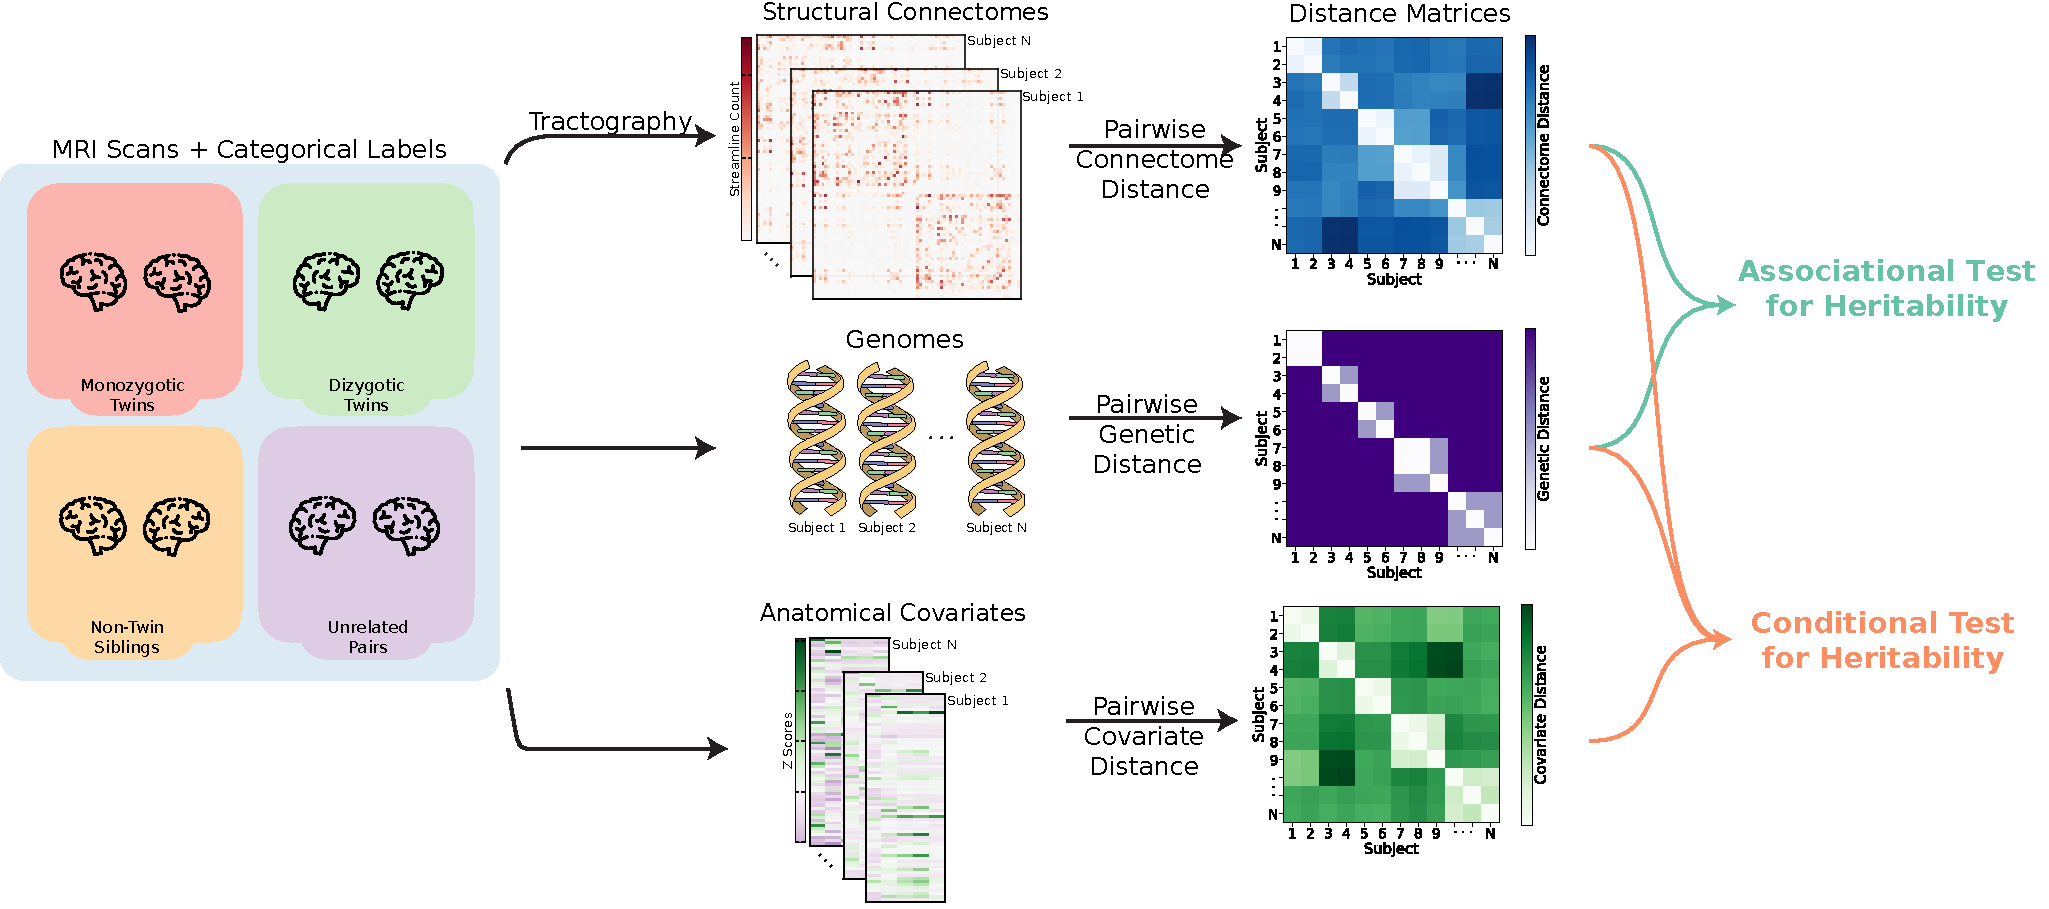
\includegraphics[width=1\linewidth]{figures/herit/framework.pdf}
  \caption
  [Overview of the framework for measuring heritability of connectomes.]
  {\textbf{Overview of the framework for measuring heritability of connectomes.} (\textit{Left}) Diffusion and structural magnetic resonance images (dMRI and sMRI) are processed to generate connectomes. Connectomes are defined on a common set of vertices using brain parcellations. Each pair of individuals has a label corresponding to whether the pair is a monozygotic twin, dizygotic twin, non-twin siblings, or unrelated (e.g. not sharing both mother and father).
  (\textit{Center left}) For each subject, connectomes and covariates are estimated from MRI scans and phenotypic data.
  (\textit{Center right}) For each modality (e.g. connectomes, genomes, and covariates), distances are computed between all possible pairs of subjects using the corresponding distance function. This results in distance matrices that are input to subsequent hypothesis tests.
  (\textit{Right}) Associational effect for connectomic heritability is measured using distance correlation ($\dcorr$). Conditional effect for connectomic heritability is measured using conditional distance correlation ($\cdcorr$). Significance tests provide evidence to reject the null that genomes and connectomes are not related.}
\label{fig:framework}
\end{figure}
